\documentclass[aspectratio=169, usepdftitle=false, xcolor={dvipsnames}, 9pt]{beamer}

\usetheme[english, notoc, coloraccent=blue]{awesome}

\title{Méthodes pour l'évaluation de l'activité cyclonique tropicale en changement climatique}
\author[William]{William Dulac}
\subtitle{Soutenance de thèse}
\email{william.dulac@meteo.fr}
\institute{Centre National de Recherches Météorologiques}
\uni{Université Paul Sabatier -- Toulouse III} 
\location{Toulouse}
\date{20 Décembre 2023}

\supervisors{Julien Cattiaux, Fabrice Chauvin}
\reporters{Jean-Philippe Duvel, Sylvie Malardel}
\examinators{Jean-Pierre Chaboureau, Christophe Menkes,\par\hspace*{16ex}Caroline Muller}

\background{include/Bolaven_2023-10-11_2300Z.jpg}

\usefonttheme[onlymath]{serif}

\begin{document}

\maketitle

\section[Introduction]{Introduction : Cyclones tropicaux}

\begin{frame}[c]
    \frametitle{Qu'est-ce qu'un cyclone tropical}
    \begin{columns}
        \begin{column}{0.45\textwidth}
            \begin{definition}
                Les phénomènes météorologiques les plus destructeurs :
                \tcblower
                \begin{itemize}
                    \item Plus de 400 000 morts et près de 300 000 blessés entre 1980 et 2009.
                    \item Deux tiers des victimes associées à seulement deux cyclones.
                \end{itemize} 
            \end{definition}
        \end{column}
        \begin{column}{0.45\textwidth}
             \begin{figure}[htpb]
                 \centering
                 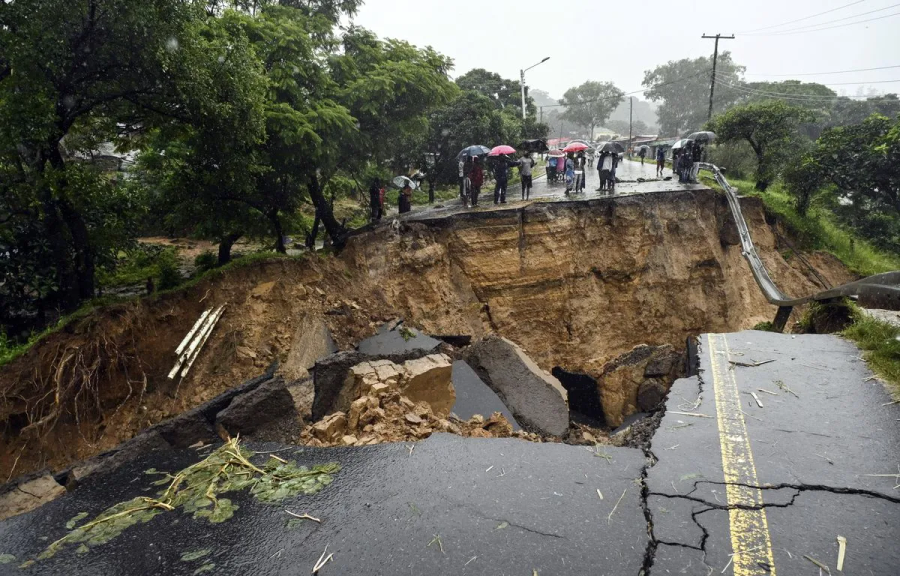
\includegraphics[width=\textwidth]{Figures/freddy_malawi_route.png}
                 \caption{Photo AP/SIPA/Thoko Chikondi}
             \end{figure}
        \end{column}
    \end{columns}
\end{frame}

\subsection{Risques associés}

\begin{frame}[t]
    \frametitle{Beaucoup de gens sont morts}
    \framesubtitle{Et deux cyclones sont responsables des 2/3}
    Foo
\end{frame}

\subsection{Consensus sur les projections futures}

\begin{frame}{Avec des équations}
    \begin{equation*}
        y(t) = x + 5
    \end{equation*}
\end{frame}


\section{Test}

\begin{frame}[t]
    \frametitle{Plan}
    \tableofcontents[currentsection]
\end{frame}

\begin{frame}[c]
    \frametitle{Avec juste un bloc}
    \framesubtitle{Voyons voir ce que ça donne}
    
    \begin{examples}[Test]
       Ceci est un bloc 
    \end{examples}
\end{frame}

\section{Test 2}

\begin{frame}[c]
    \frametitle{Avec des listes...}
    
    \begin{columns}
        \begin{column}{0.5\textwidth}
            \begin{itemize}
                \item Foo
                \item Bar
            \end{itemize}
        \end{column}
        \begin{column}{0.5\textwidth}
           \begin{enumerate}
               \item Alpha
               \item Beta
           \end{enumerate} 
        \end{column}
    \end{columns}
\end{frame}

\end{document}
